\chapter{Code source}
\label{appn}

Le code est écrit en Python et organisé en un module réutilisable
(\texttt{src/}) et des scripts d'expérimentation (\texttt{scripts/}) qui
régénèrent toutes les figures et tous les tableaux du rapport.

\section{Organisation du module \texttt{src/}}

Le module \texttt{src/} regroupe toute la logique réutilisable, indépendante de
l'expérimentation : le chargement du graphe, les structures de données, les
heuristiques et les algorithmes. La table~\ref{tab:src} en résume les fichiers, et
la table~\ref{tab:algos-files} détaille le sous-module \texttt{algorithms/}, qui
consacre un fichier à chaque algorithme.

\begin{table}[H]
  \centering
  \small
  \begin{tabular}{@{}ll@{}}
    \toprule
    Fichier & Rôle \\
    \midrule
    \texttt{network.py}        & chargement OSM, graphe compact (CSR), haversine, plus proche nœud \\
    \texttt{priority\_queue.py} & tas binaire et file à seaux de Dial \\
    \texttt{heuristics.py}     & heuristiques haversine et nulle \\
    \texttt{landmarks.py}      & sélection (\texttt{random}/\texttt{planar}/\texttt{farthest}/\texttt{avoid}), tables, borne ALT \\
    \texttt{algorithms/}       & un fichier par algorithme (voir table~\ref{tab:algos-files}) \\
    \texttt{itinerary.py}      & itinéraire lisible « tourne à gauche/droite » \\
    \texttt{interactive\_map.py} & carte HTML interactive (folium/Leaflet) \\
    \texttt{visualize.py}      & figures statiques (taches, landmarks) \\
    \texttt{animate.py}        & animation GIF de l'exploration \\
    \texttt{benchmark.py}      & harnais de banc d'essai et contrôle d'optimalité \\
    \bottomrule
  \end{tabular}
  \caption{Fichiers du module \texttt{src/} et leur rôle.}
  \label{tab:src}
\end{table}

\begin{table}[H]
  \centering
  \small
  \begin{tabular}{@{}ll@{}}
    \toprule
    Fichier & Contenu \\
    \midrule
    \texttt{base.py}          & \texttt{SearchResult}, concaténation des legs \\
    \texttt{bfs\_dfs.py}      & parcours en largeur et en profondeur \\
    \texttt{dijkstra.py}      & Dijkstra \\
    \texttt{greedy.py}        & Greedy Best-First \\
    \texttt{astar.py}         & A* générique (socle d'A*, ALT et Dijkstra) \\
    \texttt{alt.py}           & ALT \\
    \texttt{bidirectional.py} & Bi-Dijkstra et Bi-ALT (potentiel moyen) \\
    \texttt{arcflags.py}      & Arc Flags (partition $k$-means, drapeaux) \\
    \texttt{contraction.py}   & Contraction Hierarchies \\
    \bottomrule
  \end{tabular}
  \caption{Sous-module \texttt{src/algorithms/}.}
  \label{tab:algos-files}
\end{table}

\section{Scripts d'expérimentation}

Les scripts de \texttt{scripts/} sont les points d'entrée en ligne de commande.
Chacun charge le réseau, exécute les algorithmes et produit une ou plusieurs
figures et tables du rapport, à graine fixe pour être reproductible
(table~\ref{tab:scripts}).

\begin{table}[H]
  \centering
  \small
  \begin{tabular}{@{}ll@{}}
    \toprule
    Script & Produit \\
    \midrule
    \texttt{run\_multi\_stop.py}         & fig.~\ref{fig:multistop}, \ref{fig:gif-still} ; table~\ref{tab:multistop} ; itinéraire ; carte HTML \\
    \texttt{run\_benchmark.py}           & fig.~\ref{fig:benchmark} ; table~\ref{tab:benchmark} \\
    \texttt{run\_landmark\_study.py}     & fig.~\ref{fig:landmark-study}, \ref{fig:landmark-maps} ; table~\ref{tab:landmark-study} \\
    \texttt{run\_scaling\_study.py}      & fig.~\ref{fig:scaling} ; table~\ref{tab:scaling} \\
    \texttt{run\_query\_distribution.py} & fig.~\ref{fig:distribution} ; table~\ref{tab:distribution} \\
    \bottomrule
  \end{tabular}
  \caption{Scripts de \texttt{scripts/} et figures/tableaux produits.}
  \label{tab:scripts}
\end{table}

\section{Exemple d'exécution}

À titre d'exemple, le trajet fil rouge du chapitre~\ref{ch:xp} (avec sa figure,
son animation, son itinéraire détaillé et sa carte interactive) se régénère par
la commande suivante. Les étapes sont données par leur adresse ; les options
\texttt{-{}-gif}, \texttt{-{}-directions} et \texttt{-{}-map} activent
respectivement l'animation, l'itinéraire textuel et la carte HTML.

\begin{lstlisting}[language=bash]
python scripts/run_multi_stop.py \
    --stop "Place du Marechal de Lattre de Tassigny, 75016 Paris, France" \
    --stop "10 Rue d'Oradour-sur-Glane, 75015 Paris, France" \
    --stop "45 Rue d'Ulm, 75005 Paris, France" \
    --stop "60 Rue Mazarine, 75006 Paris, France" \
    --label "Dauphine" --label "PariSante" --label "ENS Ulm" --label "PSL" \
    --gif --directions --map
\end{lstlisting}

\section{Aperçu de la carte interactive}

La commande ci-dessus produit notamment une carte HTML interactive
(\texttt{results/itinerary\\\_map.html}), qui ne peut être feuilletée que dans un
navigateur. La figure~\ref{fig:htmlmap} en donne une capture d'écran : la route
optimale dessinée sur un vrai fond de plan, une couleur par leg, les marqueurs de
départ et d'étape, et un panneau récapitulatif listant les rues à suivre avec les
indications de changement de direction, autrement dit la « vue GPS » du même
chemin que celui calculé dans le chapitre~\ref{ch:xp}.

\begin{figure}[H]
  \centering
  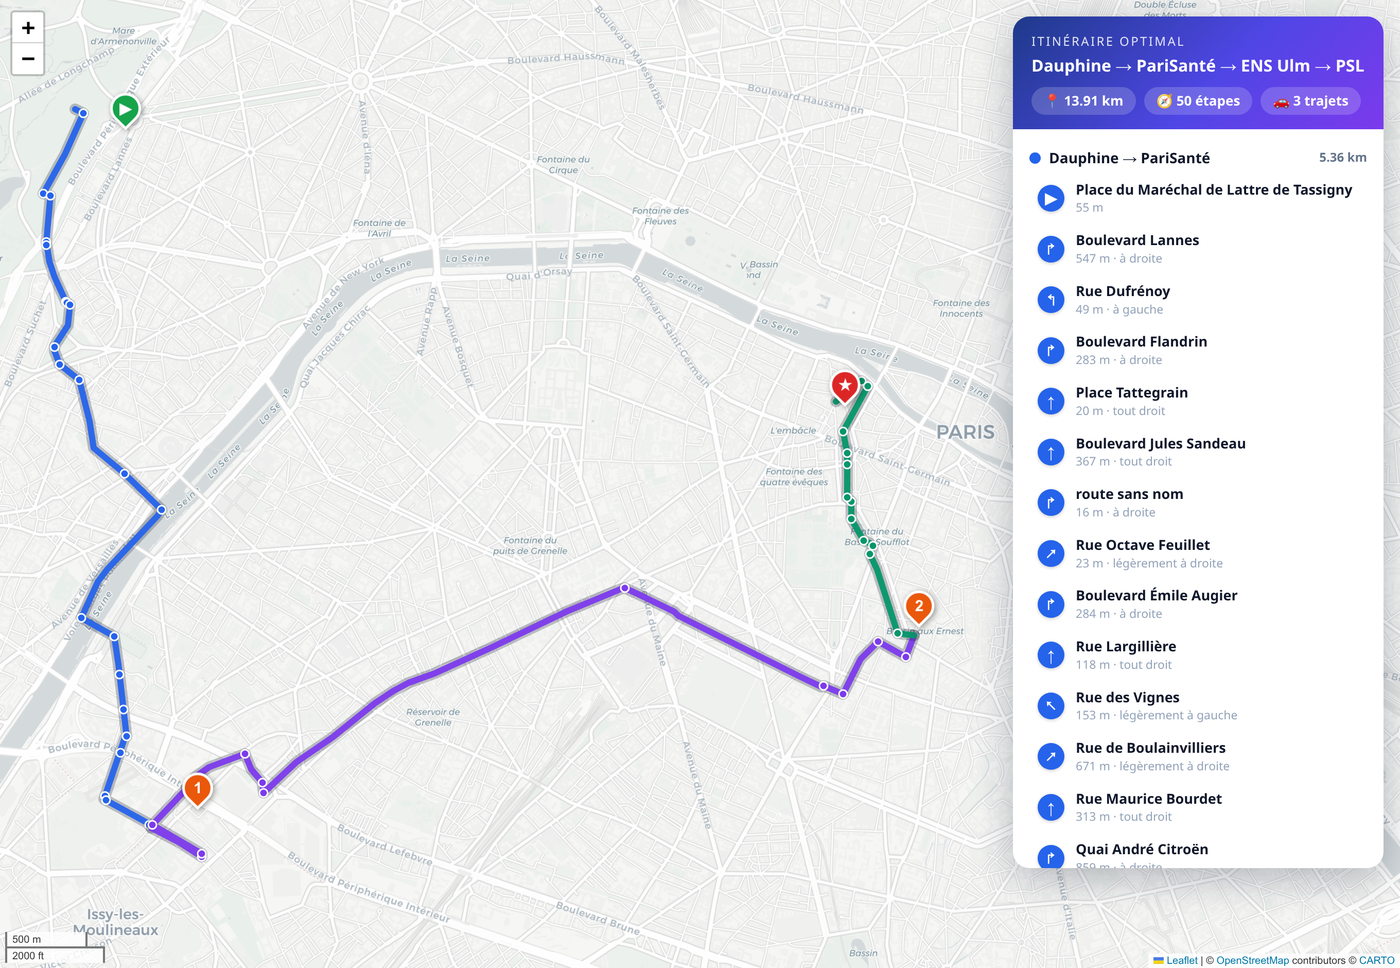
\includegraphics[width=\textwidth]{figures/itinerary_map.png}
  \caption[Capture de la carte interactive]{Capture d'écran de la carte HTML
  interactive (\texttt{itinerary\_map.html}) pour le trajet fil rouge
  Dauphine $\to$ PariSanté $\to$ ENS $\to$ PSL.}
  \label{fig:htmlmap}
\end{figure}
